%%%%%%%%%%%%%%%%%%%%%%%%%%%%%%%%%%%%%%%%%%%%%%%%%%%%%%%%%%%%%%%%%%%%%%
%%  Copyright by Wenliang Du.                                       %%
%%  This work is licensed under the Creative Commons                %%
%%  Attribution-NonCommercial-ShareAlike 4.0 International License. %%
%%  To view a copy of this license, visit                           %%
%%  http://creativecommons.org/licenses/by-nc-sa/4.0/.              %%
%%%%%%%%%%%%%%%%%%%%%%%%%%%%%%%%%%%%%%%%%%%%%%%%%%%%%%%%%%%%%%%%%%%%%%

\newcommand{\commonfolder}{../../common-files}

\documentclass[11pt]{article}

\usepackage[most]{tcolorbox}
\usepackage{times}
\usepackage{epsf}
\usepackage{epsfig}
\usepackage{amsmath, alltt, amssymb, xspace}
\usepackage{wrapfig}
\usepackage{fancyhdr}
\usepackage{url}
\usepackage{verbatim}
\usepackage{fancyvrb}
\usepackage{adjustbox}
\usepackage{listings}
\usepackage{color}
\usepackage{subfigure}
\usepackage{cite}
\usepackage{sidecap}
\usepackage{pifont}
\usepackage{mdframed}
\usepackage{textcomp}
\usepackage{enumitem}
\usepackage{hyperref}


% Horizontal alignment
\topmargin      -0.50in  % distance to headers
\oddsidemargin  0.0in
\evensidemargin 0.0in
\textwidth      6.5in
\textheight     8.9in 

\newcommand{\todo}[1]{
\vspace{0.1in}
\fbox{\parbox{6in}{TODO: #1}}
\vspace{0.1in}
}


\newcommand{\unix}{{\tt Unix}\xspace}
\newcommand{\linux}{{\tt Linux}\xspace}
\newcommand{\minix}{{\tt Minix}\xspace}
\newcommand{\ubuntu}{{\tt Ubuntu}\xspace}
\newcommand{\setuid}{{\tt Set-UID}\xspace}
\newcommand{\openssl} {\texttt{openssl}}


\pagestyle{fancy}
\lhead{\bfseries SEED Labs}
\chead{}
\rhead{\small \thepage}
\lfoot{}
\cfoot{}
\rfoot{}


\definecolor{dkgreen}{rgb}{0,0.6,0}
\definecolor{gray}{rgb}{0.5,0.5,0.5}
\definecolor{mauve}{rgb}{0.58,0,0.82}
\definecolor{lightgray}{gray}{0.90}


\lstset{%
  frame=none,
  language=,
  backgroundcolor=\color{lightgray},
  aboveskip=3mm,
  belowskip=3mm,
  showstringspaces=false,
%  columns=flexible,
  basicstyle={\small\ttfamily},
  numbers=none,
  numberstyle=\tiny\color{gray},
  keywordstyle=\color{blue},
  commentstyle=\color{dkgreen},
  stringstyle=\color{mauve},
  breaklines=true,
  breakatwhitespace=true,
  tabsize=3,
  columns=fullflexible,
  keepspaces=true,
  escapeinside={(*@}{@*)}
}

\newcommand{\newnote}[1]{
\vspace{0.1in}
\noindent
\fbox{\parbox{1.0\textwidth}{\textbf{Note:} #1}}
%\vspace{0.1in}
}


%% Submission
\newcommand{\seedsubmission}{
Debe enviar un informe de laboratorio detallado, con capturas de pantalla, para describir lo que ha hecho y lo que ha observado.
También debe proporcionar una explicación a las observaciones que sean interesantes o sorprendentes.
Enumere también los fragmentos de código más importantes seguidos de una explicación. No recibirán créditos aquellos fragmentos de códigos que no sean explicados.}

%% Book
\newcommand{\seedbook}{\textit{Computer \& Internet Security: A Hands-on Approach}, 2nd
Edition, by Wenliang Du. Para más detalles \url{https://www.handsonsecurity.net}.\xspace}

%% Videos
\newcommand{\seedisvideo}{\textit{Internet Security: A Hands-on Approach},
by Wenliang Du. Para más detalles \url{https://www.handsonsecurity.net/video.html}.\xspace}

\newcommand{\seedcsvideo}{\textit{Computer Security: A Hands-on Approach},
by Wenliang Du. Para más detalles \url{https://www.handsonsecurity.net/video.html}.\xspace}

%% Lab Environment
\newcommand{\seedenvironment}{Este laboratorio ha sido testeado en nuestra imagen pre-compilada de una VM con Ubuntu 16.04, que puede ser descargada del sitio oficial de SEED.\xspace}

\newcommand{\seedenvironmentA}{Este laboratorio ha sido testeado en nuestra imagen pre-compilada de una VM con Ubuntu 16.04, que puede ser descargada del sitio oficial de SEED.\xspace}

\newcommand{\seedenvironmentB}{Este laboratorio ha sido testeado en nuestra imagen pre-compilada de una VM con Ubuntu 20.04, que puede ser descargada del sitio oficial de SEED .\xspace}

\newcommand{\seedenvironmentC}{Este laboratorio ha sido testeado en nuestra imagen pre-compilada de una VM con Ubuntu 20.04, que puede ser descargada del sitio oficial de SEED. Sin embargo, la mayoría de nuestros laboratorios pueden ser realizados en la nube para esto Ud. puede leer nuestra guía que explica como crear una VM de SEED en la nube.\xspace}

\newcommand{\seedenvironmentAB}{
Este laboratorio ha sido testeado en nuestras imagenes pre-compiladas de una VM con Ubuntu 16.04 y otra con Ubuntu 20.04, que pueden ser descargadas del sitio oficial de SEED.\xspace}

\newcommand{\nodependency}{Dado que utilizamos contenedores para configurar el entorno de laboratorio, este laboratorio no depende estrictamente de la VM de SEED. Puede hacer este laboratorio utilizando otras máquinas virtuales, máquinas físicas o máquinas virtuales en la nube.\xspace}

\newcommand{\adddns}{You do need to add the required IP address mapping to
the \texttt{/etc/hosts} file.\xspace}






\newcommand{\seedlabcopyright}[1]{
\vspace{0.1in}
\fbox{\parbox{6in}{\small Copyright \copyright\ {#1}\ \ by Wenliang Du.\\
      Este trabajo se encuentra bajo licencia Creative Commons.
       Attribution-NonCommercial-ShareAlike 4.0 International License.
       Si ud. remezcla, transforma y construye a partir de este material,
       Este aviso de derechos de autor debe dejarse intacto o reproducirse de una manera que sea razonable para el medio en el que se vuelve a publicar el trabajo.
       }}
\vspace{0.1in}
}





\newcommand{\firewallFigs}{./Figs}
\lhead{\bfseries SEED Labs -- Laboratorio de Evasión de Firewall}

\begin{document}



\begin{center}
{\LARGE Laboratorio de Evasión de Firewall: Bypasseando Firewalls usando VPN}
\end{center}


\seedlabcopyright{2018}

\newcounter{task}
\setcounter{task}{1}
\newcommand{\tasks} {\bf {\noindent (\arabic{task})} \addtocounter{task}{1} \,}


% *******************************************
% SECTION
% ******************************************* 
\section{Descripción}

Organizaiones, Internet Service Providers (ISPs) y paises a menudo bloquean el acceso a determinados sitios externos a sus usuarios internos. Esto es llamado filtrado de salida o egress filtering.
Por ejemplo, para prevenir distracción en horarios laborales, muchas companias configuran la salida de sus firewalls para bloquear sitios de redes sociales, por lo que sus empleados no podrán acceder a estos dentro de la red interna. Por razones políticas, muchos países configurar filtrados de salida en sus ISPs para bloquear a su gente el acceso a determinados sitios foráneos. Desafortunadamente, estos firewalls pueden ser fácilmente bypasseados y existen servicios/productos que ayudan a los usuarios bypassear estos firewalls, estas soluciones están a la alcance de todos. La tecnología más usada para bypassear estos filtrados de salida son las Virtual Private Network (VPN).
Esta tecnología es ampliamente usada por usuarios que poseen smartphones y que son afectados por este tipo de bloqueo; existen muchas aplicaciones VPN (para Android, iOs y otras plataformas) que ayudan a los usuarios a evadir estas reglas de filtrado que se aplican en los firewalls.


El objetivo de este laboratorio es que los estudiantes vean como funciona una VPN y como una VPN puede ayudar a bypassear los filtrados de salida de un firewall.
En este Laboratorio, implementaremos una VPN muy simple que usaremos para bypassear firewalls. Una VPN típica depende de dos piezas: IP tunneling y el cifrado. El tunneling es esencial ya que será quien nos ayude a byppasear firewalls; el cifrado es para proteger el contenido del tráficos que viaja a través del Túnel de la VPN.
Por un tema de simplicidad, en este laboratorio solamente nos centramos en el tunneling, por lo que el tráfico dentro de nuestro Túnel no estará cifrado. Tenemos otro laboratorio sobre VPN en donde cubrimos tunneling y cifrado. Si los lectores están interesados, pueden trabajar sobre este laboratorio para aprender como construir una VPN completa. En este Laboratorio solamente nos centramos en como usar un Túnel VPN para bypassear firewalls.

Este laboratorio cubre los siguientes tópicos:

\begin{itemize}[noitemsep]
\item Firewall
\item VPN
\end{itemize}


\paragraph{Lectura y Videos.}
Para una cobertura más detallada sobre firewalls, técnicas de evasión y VPN puede consultar:

\begin{itemize}
\item Capítulos 17 y 19 del libro de SEED, \seedbook
\item Secciones 8 y 9 del curso de SEED en Udemy, \seedisvideo
\end{itemize}


\paragraph{Entorno de Laboratorio.} \seedenvironmentB
 


% *******************************************
% SECTION
% ******************************************* 
\section{Tareas del Laboratorio}




% -------------------------------------------
% SUBSECTION
% ------------------------------------------- 
\subsection{Tarea 1: Setup de la Máquina Virtual}

Necesitamos dos máquinas, una dentro del firewall y la otra fuera del firewall. El objetivo es ayudar a la máquina que se encuentra dentro del firewall que pueda visitar sitios bloqueados por el firewall.
Las máquinas que usaremos serán, VM1 y VM2, estas máquinas se suponen conectadas a internet a través de routers. Este setup puede requiera más de dos Máquinas Virtuales.
Para hacer todo más sencillo, usaremos una LAN para emular la conexión a Internet.
Básicamente, conectaremos VM1 y VM2 a la LAN usando un adaptor de \texttt{NAT Network}. 
La Figura describe el setup de nuestro laboratorio.


\begin{figure}[htb]
  \begin{center}
    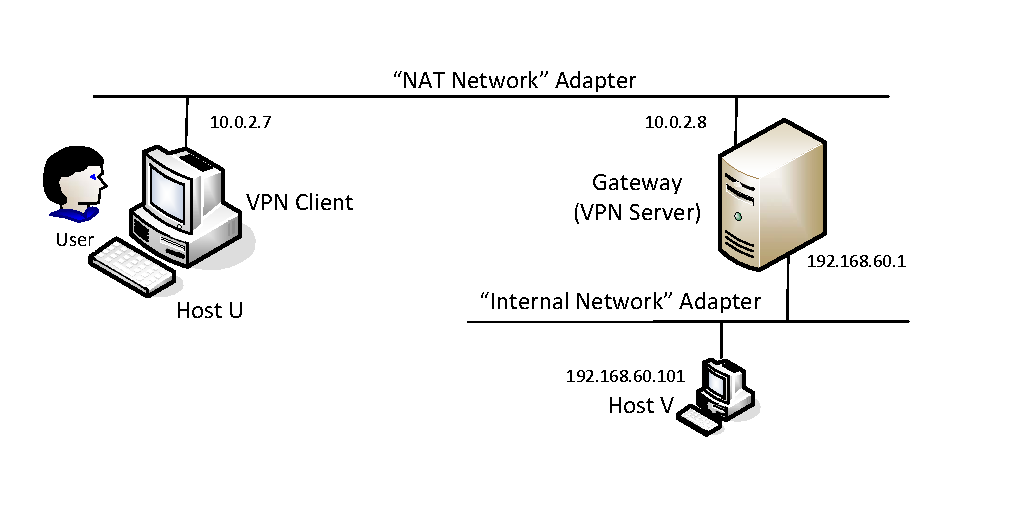
\includegraphics[width=0.9\textwidth]{\firewallFigs/Host2Gateway.pdf}
  \end{center}
  \caption{Setup del Laboratorio}
  \label{vpn_firewall:fig:labsetup}
\end{figure}



% -------------------------------------------
% SUBSECTION
% ------------------------------------------- 
\subsection{Tarea 2: Setup del Firewall}

En esta tarea, ud. hara el setup del firewall en la VM1 para bloquear el acceso a un sitio web. Debe asegurarse que la dirección IP de este sitio web sea fija o este dentro de un rango fijo; de otra forma puede terminar bloqueando por completo el sitio web. Por favor vea el laboratorio de Firewall para detalles en como bloquear sitios web.

En el mundo real, un firewall debería de correr en una máquina separada, no en VM1. Para minimizar el números de VMs usadas en el laboratorio, pondremos el firewall en VM1. Configurar un firewall en VM1 requiere de privilegios de superusuario como así también lo requiere la configuración del Túnel VPN. Uno podría decir si contamos con privilegios de superusuario, porque no podemos desactivar el firewall en VM1 y listo. Este es un buen argumento, pero tenga en cuenta, que estamos poniendo el firewall en VM1 porque no queremos crear otra VM en el entorno de laboratorio. Además, aunque cuente con privilegios de superusuario en VM1, no le es permitido usar ese privilegio para reconfigurar el firewall. Ud. deberá de usar una VPN para bypassearlo.

A diferencia de situar el firewall en una máquina externa, poner el firewall en VM1 tiene un pequeño inconveniente con el cual necesitamos convivir. Cuando hacemos el setup del firewall para bloquear paquetes, necesitamos asegurarnos de no bloquear los paquetes que vienen de la interfaz virtual usada por la VPN o nuestra VPN no será capaz de obtener los paquetes. Además, no podemos setear la regla del firewall antes del routing o setearla  en la interfaz virtual. Necesitamos setear la regla en la interfaz de red real de VM1, para no afectar a los paquetes que van hacia la interfaz virtual. El siguiente comando bloquea todo el tráfico hacia la red \texttt{93.184.216.0/24}  (\texttt{example.com}).


\begin{lstlisting}
$ sudo iptables -A OUTPUT -o enp0s3 -d 93.184.216.0/24 -j DROP
\end{lstlisting}

Por favor identifique el sitio web que quiere bloquear, haga el setup del firewall y demuestre que su firewall está funcionando y la dirección IP que esta bloqueando no se puede alcanzar. Provea capturas de pantalla en su informe del laboratorio.

% -------------------------------------------
% SUBSECTION
% ------------------------------------------- 
\subsection{Tarea 3: Bypasseando el Firewall usando VPN}

La idea de usar una VPN para bypassear un firewall es ilustrada en la Figura \ref{vpn_firewall:fig:bypassing}. 
Establecemos un Túnel VPN entre VM1 (Cliente VPN) y VM2 (Servidor VPN).
Cuando un usuario trata de acceder al sitio bloqueado, el tráfico no viajará directo a través del adaptador de red, porque será bloqueado. En vez de esto, los paquetes que se dirigen al sitio bloqueado desde VM1 serán enrutados hacia el Túnel VPN y llegarán a VM2. Una vez que estos llegan ahí, VM2 los enrutará hacia su destino final.
Cuando la respuestas de los paquetes lleguen de regreso, regresarán hacia VM2, que redireccionará los paquetes hacia el Túnel VPN y eventualmente los paquetes volverán a VM1. Así es como una VPN ayuda a bypassear firewalls.

\begin{figure}[htb]
\begin{center}
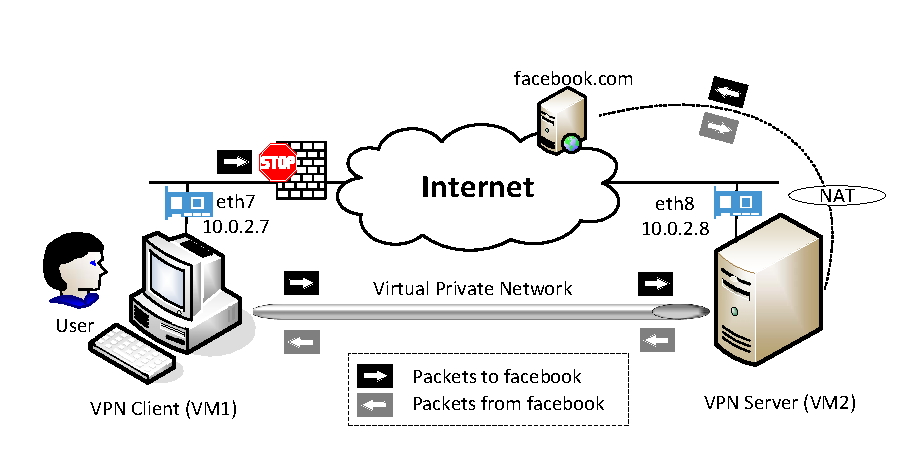
\includegraphics[width=1.0\textwidth]{\firewallFigs/BypassingFirewall.pdf}
\end{center}
\caption{Bypasseando Firewall usando una VPN}
\label{vpn_firewall:fig:bypassing}
\end{figure}
 
Hemos creado un programa VPN de ejemplo, incluídos un programa cliente (\texttt{vpnclient}) y un programa servidor (\texttt{vpnserver}), ambos pueden ser descargados del sitio oficial del laboratorio. Estos programas VPN son muy simples y solamente establecen un Túnel VPN entre el cliente y el servidor; no cifra el tráfico del Túnel.
El programa es explicado en detalle en el libro de SEED (Capítulo VPN).


\begin{figure}[htb]
\begin{center}
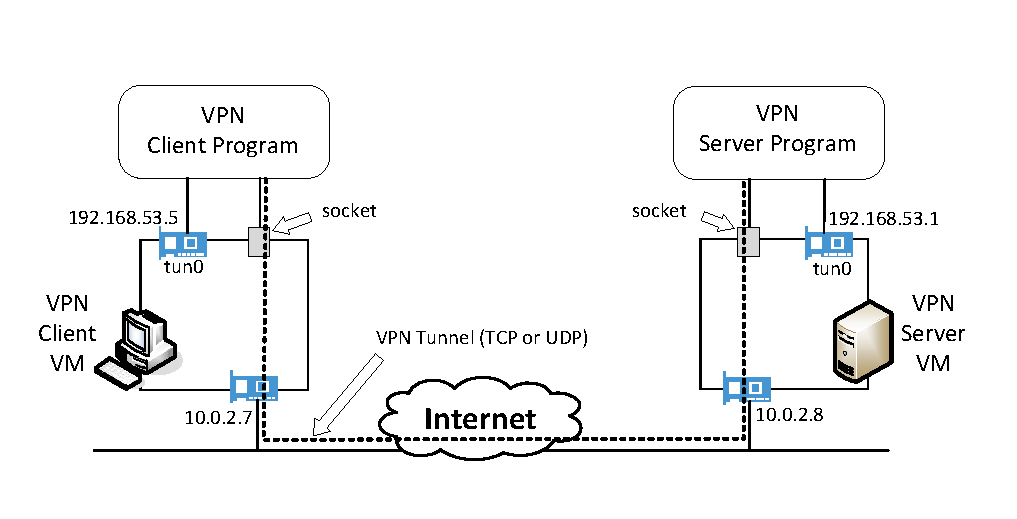
\includegraphics[width=0.9\textwidth]{\firewallFigs/ClientServerTunnel.pdf}
\end{center}
\caption{Cliente y Servidor VPN}
\label{vpn_firewall:fig:client_server}
\end{figure}

Los programas \texttt{vpnclient} y \texttt{vpnserver} son los dos puntos finales del Túnel VPN. Ellos se comunican entre sí por medio TCP o UDP a través de sockets, esto es ilustrado en la Figura \ref{vpn_firewall:fig:client_server}. En nuestro código de ejemplo, elegimos usar UDP por un tema de simplicidad. La línea punteada entre el cliente y el servidor demarca el camino para el Túnel VPN.
Los programas del cliente y servidor VPN se conectan al sistema de hosting a través de la interfaz TUN, a través de la cual ellos hacen dos cosas: (1) obtienes los paquetes IP del sistema de hosting, por lo que los paquetes pueden ser enviados a través del Túnel, (2) obtiene los paquetes IP desde el Túnel y los forwardea hacia el sistema de hosting, el cual forwardeará los paquetes hacia su destino final.
El siguiente procedimiento describe como crear un Túnel VPN usando los programas \texttt{vpnclient} y \texttt{vpnserver}.


\paragraph{Paso 1: Iniciar el Servidor VPN.}
Primer iniciamos el servidor VPN ejecutando \texttt{vpnserver} en la máquina virtual del servidor.
Después de que el programa se ejecute, aparecerá una interfaz virtual de red TUN en el sistema (puede verla usando el comando \texttt{"ifconfig -a"}; en la mayoría de los sistema el nombre de esta interfaz será \texttt{tun0} pero puede ser que sea diferente, sea como sea será \texttt{tunX} donde \texttt{X} es un número).
Esta nueva interfaz no está configurada todavía, por lo que necesitamos hacerlo, asignándole una dirección IP. Usaremos \texttt{192.168.53.1} para esta interfaz, pero puede usar otra IP.

Ejecute los siguientes comandos. El primer comando iniciará el programa servidor, el segundo comando asignará la dirección IP a la interfaz \texttt{tun0} y la activará. Debería de notar que el primer comando bloqueará y se quedará a la espera por conexiones, por lo que debemos de correr el segundo comando en una nueva ventana.


\begin{lstlisting}
$ sudo ./vpnserver

Run the following command in another window:
$ sudo ifconfig tun0 192.168.53.1/24 up
\end{lstlisting}

Al menos que se configura de una forma especial, una máquina actuará como host y no como gateway. El servidor VPN necesita forwardear los paquetes hacia otros destinos, por lo que necesita funcionar como un gateway. Necesitamos activar el IP forwarding para que la máquina se comporte como un gateway.
IP Forwarding puede ser activado usando el siguiente comando:


\begin{lstlisting}
$ sudo sysctl net.ipv4.ip_forward=1
\end{lstlisting}


\paragraph{Paso 2: Iniciar el Cliente VPN.} 
Procederemos a ejecutar el cliente VPN en la máquina virtual cliente. Correremos el siguiente comando en la máquina. El primer comando se encargará de conectar al cliente con el servidor VPN que se encuentra corriendo en {\tt 10.0.2.8}. Este comando será bloqueante por lo que necesitamos abrir otra ventana para configurar la interfaz \texttt{tun0} creada por el cliente VPN.
A la interfaz \texttt{tun0} le asignaremos la IP \texttt{192.168.53.5} (Puede seleccionar otra IP si desea).


\begin{lstlisting}
On VPN Client VM:
$ sudo ./vpnclient 10.0.2.8

Run the following command in a different window
$ sudo ifconfig tun0 192.168.53.5/24 up
\end{lstlisting}



\paragraph{Paso 3: Configurando el Routing en las Máquinas Cliente y Servidor.}
Después de realizar los pasos anteriores, el Túnel será establecido.
Antes de poder usar el Túnel, necesitamos configurar los caminos de enrutamiento en las máquinas del cliente y del servidor para así poder direccionar el tráfico que nos interesa a través del Túnel.
Podemos usar el comando \texttt{route} para agregar entradas. El siguiente ejemplo muestra como enrutar los paquetes de \texttt{10.20.30.0/24} hacia la interfaz \texttt{eth0}.


\begin{lstlisting}
$ sudo route add -net 10.20.30.0/24 eth0
\end{lstlisting}

Para bypassear los firewwalls en la máquina virtual del cliente, necesita configurar las entradas de enrutamiento que corresponden, de esta forma el tráfico que se dirige hacia el sitio bloqueado será enrutado hacia la VPN. Necesita pensar que entradas de enrutamiento agregar para bypassear el firewall.



\paragraph{Paso 4: Setup del NAT en la Máquina Virtual del Servidor.}
Cuando el destino final envía los paquetes de regreso a los usuarios, el paquete será enviado hacia el servidor VPN primero (piense el porque y escriba su respuesta en el informe del laboratorio). El retorno del paquete llegará al adaptador NAT del servidor VPN en primera instancia,porque las direcciones de IPs de origen de todo los paquetes salientes de la máquina virtual del servidor se cambian a la dirección IP externa del NAT (que es básicamente la IP de la máquina host de nuestro setup). Usualmente, el NAT reemplazará la IP de destino con la IP del paquete original (en nuestro caso \texttt{192.168.53.5}) y se la devolverá a quien sea el dueño de esa dirección IP. Desafortunadamente, aquí tenemos un problema.

Antes que la NAT envíe el paquete, necesita conocer la dirección MAC de la máquina que es la dueña de la dirección IP \texttt{192.168.53.5}, por lo que enviará una petición ARP. Nuestra red privada es virtual y esta dirección IP pertenece a la interfaz \texttt{tun0} del cliente VPN.
Además \texttt{192.168.53.5} no recibirá la petición ARP (incluso si esto pasará, no serviría de nada). El NAT rechazará el paquete, porque el receptor no existe.

El receptor actual debería de ser la máquina virtual del servidor VPN, aunque no sea dueña de la IP \texttt{192.168.53.5}. Si podemos configurar el NAT como un gateway, podemos pedirle a el NAT que enrute los paquetes para \texttt{192.168.53.5}  hacia el servidor VPN, el cual eventualmente entregará los paquetes a través del Túnel al cliente VPN. Sin embargo, no hemos encontrado la forma de como configurar el NAT como un gateway en VirtualBox, hemos trabajado en dos soluciones.
Una idea es ``engañar'' a la NAT haciendole creer que la dirección MAC de \texttt{192.168.53.5} la máquina del servidor VPN, por lo que el paquete será entregado al servidor VPN por el NAT. Podemos lograr esto usando ARP cache poisoning en la NAT, básicamente haciéndole saber a la NAT de antemano sobre la dirección MAC de \texttt{192.168.53.5}.

Una mejor solución para esta limitación del NAT es crear otra NAT en la máquina virtual del servidor, por lo que todos los paquetes que salen del servidor tendrán la dirección IP de la máquina virtual como dirección IP de origen.
Para salir a la Internet, estos paquetes viajarán a través de la otra NAT, que es provista por VirtualBox, pero dado que la IP de origen es la máquina virtual del servidor, la segunda NAT no tendrá problemas para retransmitir los paquetes devueltos desde la Internet hacia la máquina virtual del servidor. Usando esta solución, no tenemos la necesidad de usar ARP cache poisoning para ``engañar'' a la NAT. Los siguientes comandos pueden ser usados para activar la NAT en la máquina virtual del servidor (en su caso, el nombre del adaptador \texttt{NAT Network} puede que no se llame \texttt{enp0s3}; sólo necesita encontrar el verdadero nombre en su máquina virtual):

    
\begin{lstlisting}
$ sudo iptables -t nat -A POSTROUTING -j MASQUERADE -o enp0s3
\end{lstlisting}
    

\paragraph{Demostración.}
Si ud. ha realizado los pasos anteriores de manera correcta, debería de poder bypassear el firewall. Debería de mostrar que puede acceder al sitio bloqueado desde la máquina virtual del cliente a través de la VPN. Su solución no solamente debería de funcionar para tráfico web sino para todo tipo de tráfico. Por ejemplo, si la máquina bloqueada hace \texttt{telnet} al servidor bloqueado, debería de poder establecer una conexión \texttt{telnet} desde la máquina cliente.

En su informe del laboratorio, debe de proporcionar evidencia que muestre que su tráfico pasó por el Túnel VPN y no por ``puertas laterales''. La mejor forma de mostrarlo es capturar el tráfico de red usando Wireshark y describir el camino de sus paquetes usando el tráfico capturado. Sin esta evidencia, no tendremos idea si su éxito se debió a un firewall mal configurado (es decir el sitio web que se supone bloqueado no lo está) o por una VPN mal configurada.

% *******************************************
% SECTION
% ******************************************* 
\section{Informe del Laboratorio}

%%%%%%%%%%%%%%%%%%%%%%%%%%%%%%%%%%%%%%%%

Debe enviar un informe de laboratorio detallado, con capturas de pantalla, para describir lo que ha hecho y lo que ha observado.
También debe proporcionar una explicación a las observaciones que sean interesantes o sorprendentes.
Enumere también los fragmentos de código más importantes seguidos de una explicación. No recibirán créditos aquellos fragmentos de códigos que no sean explicados.
%%%%%%%%%%%%%%%%%%%%%%%%%%%%%%%%%%%%%%%%

\section*{Agradecimientos}

Este documento ha sido traducido al Español por Facundo Fontana


\end{document}


